%#######################################
% Original: Oktober.2011; Prof. Dr. Martin Grüttmüller, FIM
% Last Edit: Dezember.2021; M.Eng. Mario Hoffmann, Fakultät DIT
% Reimport: April.2022; Prof. Dr. Jean-Alexander Müller, Fakultät Informatik und Medien
%#######################################

%!TEX TS-program = lualatex
%!TEX encoding = UTF-8 Unicode
%!TEX root = MusterAbschlussarbeit.tex
%!TEX spellcheck = de_DE
%!BIB program = biber

\documentclass[a4paper,12pt,numbers=noenddot,parskip,toc=flat,toc=listof,toc=bibliography,twoside=false,captions=tableheading]{scrbook}

%##########################################################
% Dokumentenangaben
%##########################################################
%########## INB
%\newcommand{\abschlussarbeit}{Bachelorarbeit}
%\newcommand{\studiengang}{Informatik}
%\newcommand{\studienganggrad}{Bachelor of Science}
%########## INM
\newcommand{\abschlussarbeit}{Bachelorarbeit}
\newcommand{\studiengang}{Informatik}
\newcommand{\studienganggrad}{Bachelor of Science}
%########## EoStudiengang
\newcommand{\autor}{Tony Lenz}
\newcommand{\geburtsort}{Leipzig}
\newcommand{\geburtstag}{07.01.1993}
\newcommand{\titel}{Evaluierung von Reinforcement Learning-Algorhitmen anhand eines Würfelspiels in Unity}
% Falls kein Untertitel, einfach leer lassen
\newcommand{\subtitel}{}
\newcommand{\fakultät}{Informatik und Medien}
\newcommand{\erstgutachter}{Prof. Dr.-Ing. Müller ERSTGUTACHTER}
\newcommand{\instituteErstgutachter}{HTWK Leipzig}
\newcommand{\zweitgutachter}{Prof. Dr.-Ing. Bleymehl ZWEITGUTACHTER}
\newcommand{\instituteZweitgutachter}{HTWK Leipzig}
\newcommand{\ort}{Leipzig}

% Im Fall eines Themas seitens eines Praxispartners --> Sperrvermerke sind genehmigungs-
% pflichtig!
%\newcommand{\betrieb}{BETRIEB}

%##########################################################
% Einbinden aller Pakete etc.
%##########################################################

%!TeX root = ./../MusterAbschlussarbeit.tex


%##########################################################
% Pakete - Stil, Sprache und Schriftart
%##########################################################
\usepackage[UKenglish,ngerman]{babel}
\usepackage[T1]{fontenc}
\usepackage[osf,scale=1.15]{sourcesanspro}
\usepackage{csquotes}
\usepackage[backend=biber,sorting=none,bibencoding=utf8]{biblatex}
\addbibresource{MusterBachelorArbeitBib.bib}
\usepackage[headsepline]{scrlayer-scrpage}
\usepackage{fontspec}
\setcounter{tocdepth}{\subsubsectiontocdepth}
\addtokomafont{chapterentry}{\bfseries}
\usepackage[onehalfspacing]{setspace}
%## #### #### ####### ###
\usepackage[absolute, overlay]{textpos}
\usepackage{svg}
%\DeclareGraphicsExtensions{.png,.jpg,.gif,.pdf,.svg}
%\renewcommand\includesvg[2][]{\includegraphics{#2}}

\AtBeginDocument{%
	\providecaptionname{ngerman}{\lstlistlistingname}{Quellcodeverzeichnis}
	\providecaptionname{ngerman}{\lstlistingname}{Quellcode}
}

%##########################################################
% Pakete - Grafisches Elemente und Farben
%##########################################################
\usepackage{graphicx}
\usepackage{xcolor}

\providecommand{\keywords}[1]{\textbf{\textit{Keywords:}} #1}

%############ HTWK Farben #################
\xdefinecolor{htwkGelb}{rgb}{0.996,0.925,0}
\xdefinecolor{htwkGrau}{rgb}{0.945,0.945,0.945}
\xdefinecolor{htwkBlau}{rgb}{0,0.273,0.597}
\xdefinecolor{htwkMagenta}{rgb}{0.894,0,0.488}
\xdefinecolor{htwkRot}{rgb}{0.894,0.1875,0.035}
\xdefinecolor{htwkGruen}{rgb}{0,0.586,0.304}
\xdefinecolor{htwkCyan}{rgb}{0,0.617,0.886}
\xdefinecolor{codegreen}{rgb}{0,0.6,0}
%######## Legen Sie die Farbe fest #####
% htwkBlau, htwkGruen, htwkRot, htwkCyan, htwkGelb, htwkMagenta, htwkGrau
\newcommand{\farbe}{htwkBlau}
%#########################################

%Linkformatierung
\usepackage[
	    colorlinks=true,
	    urlcolor=htwkBlau,
	    citecolor=htwkBlau,
		pdftitle={\titel},
		pdfauthor={\autor},
		breaklinks=true,
		hidelinks
]{hyperref}

%##########################################################
% Pakete - Zusätzliche
%##########################################################

\usepackage{listings}
\usepackage{scrhack}
\usepackage{microtype}
\usepackage{acro}

%##########################################################
% Code Snippet Definitionen
%##########################################################
\newcommand\digitstyle{\color{purple}}
\makeatletter
\newcommand{\ProcessDigit}[1]
{%
  \ifnum\lst@mode=\lst@Pmode\relax%
   {\digitstyle #1}%
  \else
    #1%
  \fi
}

\lstdefinestyle{MyStyle}{
	basicstyle=\footnotesize\sffamily,
	keywordstyle=\color{blue},
	commentstyle=\color{codegreen},
	stringstyle=\color{orange!80!black},
	morecomment=[l]{//},
	morecomment=[l]{/*}{*/},
	morestring=[b]",
	morestring=[b]',
	breakatwhitespace=false,         
    breaklines=true,                 
    keepspaces=true,
	showspaces=false,                
    showstringspaces=false,
    showtabs=false,                  
    tabsize=2,
	numbers=left,
	numberstyle=\tiny,
	frameround=tttt,
	frame=trbl,
	columns=fullflexible,
	xleftmargin=0.03\linewidth,
	xrightmargin=0.01\linewidth,
	inputencoding=utf8,
}

\lstset{
	style=MyStyle,
	literate=%
    {0}{{{\ProcessDigit{0}}}}1
    {1}{{{\ProcessDigit{1}}}}1
    {2}{{{\ProcessDigit{2}}}}1
    {3}{{{\ProcessDigit{3}}}}1
    {4}{{{\ProcessDigit{4}}}}1
    {5}{{{\ProcessDigit{5}}}}1
    {6}{{{\ProcessDigit{6}}}}1
    {7}{{{\ProcessDigit{7}}}}1
    {8}{{{\ProcessDigit{8}}}}1
    {9}{{{\ProcessDigit{9}}}}1
}

%!TeX root = ./../MusterAbschlussarbeit.tex

%##########################################################
% Inhalt
%##########################################################

\DeclareAcronym{htwk}{
    short = HTWK,
    long = Hochschule für Technik{,} Wirtschaft und Kultur Leipzig
}

\DeclareAcronym{fim}{
    short = FIM,
    long = Fakultät Informatik und Medien
}

\DeclareAcronym{html}{
    short = HTML,
    long = Hypertext Markup Language
}

\DeclareAcronym{ftth}{
    short = FTTH,
    long = Fiber to the Home
}

\DeclareAcronym{ml}{
    short = ML,
    long = Machine Learning
}


%##########################################################
% Begin des Dokumentes
%##########################################################
\begin{document}

%!TeX root = ./../MusterAbschlussarbeit.tex

\pagestyle{scrheadings}
\clearpairofpagestyles

\ofoot[\pagemark]{\pagemark}
\ohead{\headmark}
\automark{chapter}

%!TeX root = ./../MusterAbschlussarbeit.tex

%##########################################################
% Titelseite
%##########################################################

\begin{titlepage}
	\noindent
\begin{textblock*}{4.74cm}(16.7mm,11mm)

\includegraphics[width=4.74cm]{Bilder/logos/HTWK-Fakultaetszusatz_IM_schwarz_de-eps-converted-to.pdf}
\end{textblock*}
\begin{center}

\vspace*{0.5cm}

\large
{\textsc{\Large \abschlussarbeit}}

\vspace*{0.5cm}
zur Erlangung des akademischen Grades\\[0.6cm]
\studienganggrad\\[0.6cm]
im Studiengang \studiengang\\
der Fakultät \fakultät\\
der Hochschule für Technik, Wirtschaft und Kultur Leipzig

{\LARGE \textbf{\titel}}\\
{\LARGE \textbf{-- \subtitel --}}

\end{center}

%##########################################################
% Autor/in
%##########################################################

\vspace*{2cm}
vorgelegt von: \autor \\
Geburtsort und -datum: \geburtsort, den \geburtstag \\
Abgabe: \ort, den \today



\vspace*{1cm}
\large
\begin{tabbing}
\hspace{4cm}\=\kill
Erstgutachter:  \> \erstgutachter, \\ \> \instituteErstgutachter\\ 
Zweitgutachter:  \> \zweitgutachter, \\ \> \instituteZweitgutachter
\end{tabbing} 

\begin{textblock*}{8.41cm}(18mm,268.3mm)

\includegraphics[width=8.41cm]{Bilder/logos/htwk-logo-eps-converted-to.pdf}
\end{textblock*}

\end{titlepage}


%##########################################################
% Sperrvermerk
% Ist vorher abzuklären!
%##########################################################
\pagenumbering{gobble}
%%!TeX root = ./../MusterAbschlussarbeit.tex

%##########################################################
% Inhalt
%##########################################################

\thispagestyle{empty} % no page number
\chapter*{Sperrvermerk}

\noindent
Die vorliegende Bachelorarbeit mit dem Titel \titel{} beinhaltet interne vertrauliche Informationen der Firma \betrieb{} des Autors oder patentrechtlich relevante Informationen. 

Die Weitergabe des gesperrten Inhaltes der Arbeit und eventuell beiliegender
Zeichnungen und Daten im Gesamten oder in Teilen ist grundsätzlich untersagt. Es dürfen keinerlei Kopien oder
Abschriften -- auch in digitaler Form -- gefertigt werden. 
Ausnahmen bedürfen der vorherigen schriftlichen Genehmigung der Firma \betrieb{} oder des Autors.

%Hier kommen die Unterschriften hin
\vspace{1.5cm}
\begin{tabular}{p{7cm}p{.5cm}p{7cm}}
	\dotfill & & \dotfill \\\\
	Ort, Datum, Unterschrift \erstgutachter & & Ort, Datum, Unterschrift \zweitgutachter \\
    & & \\\\
    & & \\\\
    \dotfill \\\\
    Ort, Datum, Unterschrift \autor
\end{tabular}


%##########################################################
% Eidesstaatliche Erklärung
%##########################################################
\relax 
\providecommand{\transparent@use}[1]{}
\providecommand\hyper@newdestlabel[2]{}
\@setckpt{Formalien/EidesstaatlicheErklaerung}{
\setcounter{page}{1}
\setcounter{equation}{0}
\setcounter{enumi}{0}
\setcounter{enumii}{0}
\setcounter{enumiii}{0}
\setcounter{enumiv}{0}
\setcounter{footnote}{0}
\setcounter{mpfootnote}{0}
\setcounter{part}{0}
\setcounter{chapter}{0}
\setcounter{section}{0}
\setcounter{subsection}{0}
\setcounter{subsubsection}{0}
\setcounter{paragraph}{0}
\setcounter{subparagraph}{0}
\setcounter{figure}{0}
\setcounter{table}{0}
\setcounter{tabx@nest}{0}
\setcounter{listtotal}{0}
\setcounter{listcount}{0}
\setcounter{liststart}{0}
\setcounter{liststop}{0}
\setcounter{citecount}{0}
\setcounter{citetotal}{0}
\setcounter{multicitecount}{0}
\setcounter{multicitetotal}{0}
\setcounter{instcount}{0}
\setcounter{maxnames}{3}
\setcounter{minnames}{1}
\setcounter{maxitems}{3}
\setcounter{minitems}{1}
\setcounter{citecounter}{0}
\setcounter{maxcitecounter}{0}
\setcounter{savedcitecounter}{0}
\setcounter{uniquelist}{0}
\setcounter{uniquename}{0}
\setcounter{refsection}{0}
\setcounter{refsegment}{0}
\setcounter{maxextratitle}{0}
\setcounter{maxextratitleyear}{0}
\setcounter{maxextraname}{0}
\setcounter{maxextradate}{0}
\setcounter{maxextraalpha}{0}
\setcounter{abbrvpenalty}{50}
\setcounter{highnamepenalty}{50}
\setcounter{lownamepenalty}{25}
\setcounter{maxparens}{3}
\setcounter{parenlevel}{0}
\setcounter{blx@maxsection}{0}
\setcounter{blx@maxsegment@0}{0}
\setcounter{blx@sectionciteorder@0}{0}
\setcounter{mincomprange}{10}
\setcounter{maxcomprange}{100000}
\setcounter{mincompwidth}{1}
\setcounter{afterword}{0}
\setcounter{savedafterword}{0}
\setcounter{annotator}{0}
\setcounter{savedannotator}{0}
\setcounter{author}{0}
\setcounter{savedauthor}{0}
\setcounter{bookauthor}{0}
\setcounter{savedbookauthor}{0}
\setcounter{commentator}{0}
\setcounter{savedcommentator}{0}
\setcounter{editor}{0}
\setcounter{savededitor}{0}
\setcounter{editora}{0}
\setcounter{savededitora}{0}
\setcounter{editorb}{0}
\setcounter{savededitorb}{0}
\setcounter{editorc}{0}
\setcounter{savededitorc}{0}
\setcounter{foreword}{0}
\setcounter{savedforeword}{0}
\setcounter{holder}{0}
\setcounter{savedholder}{0}
\setcounter{introduction}{0}
\setcounter{savedintroduction}{0}
\setcounter{namea}{0}
\setcounter{savednamea}{0}
\setcounter{nameb}{0}
\setcounter{savednameb}{0}
\setcounter{namec}{0}
\setcounter{savednamec}{0}
\setcounter{translator}{0}
\setcounter{savedtranslator}{0}
\setcounter{shortauthor}{0}
\setcounter{savedshortauthor}{0}
\setcounter{shorteditor}{0}
\setcounter{savedshorteditor}{0}
\setcounter{labelname}{0}
\setcounter{savedlabelname}{0}
\setcounter{institution}{0}
\setcounter{savedinstitution}{0}
\setcounter{lista}{0}
\setcounter{savedlista}{0}
\setcounter{listb}{0}
\setcounter{savedlistb}{0}
\setcounter{listc}{0}
\setcounter{savedlistc}{0}
\setcounter{listd}{0}
\setcounter{savedlistd}{0}
\setcounter{liste}{0}
\setcounter{savedliste}{0}
\setcounter{listf}{0}
\setcounter{savedlistf}{0}
\setcounter{location}{0}
\setcounter{savedlocation}{0}
\setcounter{organization}{0}
\setcounter{savedorganization}{0}
\setcounter{origlocation}{0}
\setcounter{savedoriglocation}{0}
\setcounter{origpublisher}{0}
\setcounter{savedorigpublisher}{0}
\setcounter{publisher}{0}
\setcounter{savedpublisher}{0}
\setcounter{language}{0}
\setcounter{savedlanguage}{0}
\setcounter{origlanguage}{0}
\setcounter{savedoriglanguage}{0}
\setcounter{pageref}{0}
\setcounter{savedpageref}{0}
\setcounter{textcitecount}{0}
\setcounter{textcitetotal}{0}
\setcounter{textcitemaxnames}{0}
\setcounter{biburlbigbreakpenalty}{100}
\setcounter{biburlbreakpenalty}{200}
\setcounter{biburlnumpenalty}{0}
\setcounter{biburlucpenalty}{0}
\setcounter{biburllcpenalty}{0}
\setcounter{smartand}{1}
\setcounter{bbx:relatedcount}{0}
\setcounter{bbx:relatedtotal}{0}
\setcounter{svg@param@lastpage}{0}
\setcounter{svg@param@currpage}{-1}
\setcounter{Item}{0}
\setcounter{Hfootnote}{0}
\setcounter{bookmark@seq@number}{0}
\setcounter{lstnumber}{1}
\setcounter{section@level}{0}
\setcounter{lstlisting}{0}
}


%##########################################################
% Vorwort (optional)
%##########################################################
%!TeX root = ./../MusterAbschlussarbeit.tex

%##########################################################
% Inhalt
%##########################################################
\clearpage
\chapter*{Vorwort (optional)}
In einem Vorwort können persönliche Danksagungen, Ihre eigene Motivation sowie persönliche Erkenntnisse niederschreiben. 
Inhaltliche Angaben zum Werk werden jedoch nicht gemacht. Zudem ist es möglich hier eine Gendererklärung abzugeben.
Gendererklärung:
In dieser Arbeit wird aus Gründen der besseren Lesbarkeit das generische Maskulinum verwendet. 
Weibliche und anderweitige Geschlechteridentitäten werden dabei ausdrücklich mitgemeint, soweit es für die Aussage erforderlich ist.


%##########################################################
% Abstract/Kurzfassung
%##########################################################
\relax 
\providecommand{\transparent@use}[1]{}
\providecommand\hyper@newdestlabel[2]{}
\@setckpt{Formalien/Kurzfassung}{
\setcounter{page}{1}
\setcounter{equation}{0}
\setcounter{enumi}{0}
\setcounter{enumii}{0}
\setcounter{enumiii}{0}
\setcounter{enumiv}{0}
\setcounter{footnote}{0}
\setcounter{mpfootnote}{0}
\setcounter{part}{0}
\setcounter{chapter}{0}
\setcounter{section}{0}
\setcounter{subsection}{0}
\setcounter{subsubsection}{0}
\setcounter{paragraph}{0}
\setcounter{subparagraph}{0}
\setcounter{figure}{0}
\setcounter{table}{0}
\setcounter{tabx@nest}{0}
\setcounter{listtotal}{0}
\setcounter{listcount}{0}
\setcounter{liststart}{0}
\setcounter{liststop}{0}
\setcounter{citecount}{0}
\setcounter{citetotal}{0}
\setcounter{multicitecount}{0}
\setcounter{multicitetotal}{0}
\setcounter{instcount}{0}
\setcounter{maxnames}{3}
\setcounter{minnames}{1}
\setcounter{maxitems}{3}
\setcounter{minitems}{1}
\setcounter{citecounter}{0}
\setcounter{maxcitecounter}{0}
\setcounter{savedcitecounter}{0}
\setcounter{uniquelist}{0}
\setcounter{uniquename}{0}
\setcounter{refsection}{0}
\setcounter{refsegment}{0}
\setcounter{maxextratitle}{0}
\setcounter{maxextratitleyear}{0}
\setcounter{maxextraname}{0}
\setcounter{maxextradate}{0}
\setcounter{maxextraalpha}{0}
\setcounter{abbrvpenalty}{50}
\setcounter{highnamepenalty}{50}
\setcounter{lownamepenalty}{25}
\setcounter{maxparens}{3}
\setcounter{parenlevel}{0}
\setcounter{blx@maxsection}{0}
\setcounter{blx@maxsegment@0}{0}
\setcounter{blx@sectionciteorder@0}{0}
\setcounter{mincomprange}{10}
\setcounter{maxcomprange}{100000}
\setcounter{mincompwidth}{1}
\setcounter{afterword}{0}
\setcounter{savedafterword}{0}
\setcounter{annotator}{0}
\setcounter{savedannotator}{0}
\setcounter{author}{0}
\setcounter{savedauthor}{0}
\setcounter{bookauthor}{0}
\setcounter{savedbookauthor}{0}
\setcounter{commentator}{0}
\setcounter{savedcommentator}{0}
\setcounter{editor}{0}
\setcounter{savededitor}{0}
\setcounter{editora}{0}
\setcounter{savededitora}{0}
\setcounter{editorb}{0}
\setcounter{savededitorb}{0}
\setcounter{editorc}{0}
\setcounter{savededitorc}{0}
\setcounter{foreword}{0}
\setcounter{savedforeword}{0}
\setcounter{holder}{0}
\setcounter{savedholder}{0}
\setcounter{introduction}{0}
\setcounter{savedintroduction}{0}
\setcounter{namea}{0}
\setcounter{savednamea}{0}
\setcounter{nameb}{0}
\setcounter{savednameb}{0}
\setcounter{namec}{0}
\setcounter{savednamec}{0}
\setcounter{translator}{0}
\setcounter{savedtranslator}{0}
\setcounter{shortauthor}{0}
\setcounter{savedshortauthor}{0}
\setcounter{shorteditor}{0}
\setcounter{savedshorteditor}{0}
\setcounter{labelname}{0}
\setcounter{savedlabelname}{0}
\setcounter{institution}{0}
\setcounter{savedinstitution}{0}
\setcounter{lista}{0}
\setcounter{savedlista}{0}
\setcounter{listb}{0}
\setcounter{savedlistb}{0}
\setcounter{listc}{0}
\setcounter{savedlistc}{0}
\setcounter{listd}{0}
\setcounter{savedlistd}{0}
\setcounter{liste}{0}
\setcounter{savedliste}{0}
\setcounter{listf}{0}
\setcounter{savedlistf}{0}
\setcounter{location}{0}
\setcounter{savedlocation}{0}
\setcounter{organization}{0}
\setcounter{savedorganization}{0}
\setcounter{origlocation}{0}
\setcounter{savedoriglocation}{0}
\setcounter{origpublisher}{0}
\setcounter{savedorigpublisher}{0}
\setcounter{publisher}{0}
\setcounter{savedpublisher}{0}
\setcounter{language}{0}
\setcounter{savedlanguage}{0}
\setcounter{origlanguage}{0}
\setcounter{savedoriglanguage}{0}
\setcounter{pageref}{0}
\setcounter{savedpageref}{0}
\setcounter{textcitecount}{0}
\setcounter{textcitetotal}{0}
\setcounter{textcitemaxnames}{0}
\setcounter{biburlbigbreakpenalty}{100}
\setcounter{biburlbreakpenalty}{200}
\setcounter{biburlnumpenalty}{0}
\setcounter{biburlucpenalty}{0}
\setcounter{biburllcpenalty}{0}
\setcounter{smartand}{1}
\setcounter{bbx:relatedcount}{0}
\setcounter{bbx:relatedtotal}{0}
\setcounter{svg@param@lastpage}{0}
\setcounter{svg@param@currpage}{-1}
\setcounter{Item}{0}
\setcounter{Hfootnote}{0}
\setcounter{bookmark@seq@number}{0}
\setcounter{lstnumber}{1}
\setcounter{section@level}{0}
\setcounter{lstlisting}{0}
}


%##########################################################
% Inhaltsverzeichnis
%##########################################################
\tableofcontents

%##########################################################
% Abbildungsverzeichnis
%##########################################################
\listoffigures

%##########################################################
% Tabellenverzeichnis
%##########################################################\
\listoftables

%##########################################################
% Quelltextverzeichnis
%##########################################################\
\lstlistoflistings
\clearpage

%##########################################################
% Abkürzungsverzeichnis
%##########################################################
\printacronyms[name=Abkürzungsverzeichnis, heading=chapter*]
\addcontentsline{toc}{chapter}{Abkürzungsverzeichnis}

%##########################################################
% Erstes Kapitel
%##########################################################
%!TeX root = ./../MusterAbschlussarbeit.tex

%##########################################################
% Inhalt
%##########################################################
\pagenumbering{arabic}
\chapter{Einleitung}

In der heutigen Zeit stehen wir an der Schwelle einer digitalen Revolution, in der maschinelles Lernen und künstliche Intelligenz eine immer bedeutendere Rolle spielen. Insbesondere das Gebiet des Reinforcement Learning hat in den letzten Jahren enorme Fortschritte gemacht und findet Anwendung in einer Vielzahl von Bereichen, von der Robotik bis hin zu Finanzen. Diese Entwicklung bietet aufregende Möglichkeiten, komplexe Probleme zu lösen und intelligente Systeme zu entwickeln, die in der Lage sind, eigenständig zu lernen und Entscheidungen zu treffen.

Reinforcement Learning (RL) hat bereits beeindruckende Erfolge erzielt, indem es Algorithmen entwickelt hat, die komplexe Spiele wie Go auf einem kompetitiven Niveau spielen können und sogar über menschliche Fähigkeiten hinausgehen. Darüber hinaus wurde RL erfolgreich eingesetzt, um die Effizienz und Leistung von Serverfarmen bei Unternehmen wie Google zu optimieren. Diese Anwendungen verdeutlichen die Vielseitigkeit und Leistungsfähigkeit von Reinforcement Learning bei der Bewältigung verschiedenster Herausforderungen und unterstreichen seine Fähigkeit, komplexe Probleme zu lösen und neue Lösungswege zu finden.

In dieser Bachelorarbeit liegt der Fokus auf der Implementierung und dem Training eines Reinforcement Learning-Agenten für das Würfelspiel 'Noch mal'. 'Noch mal' ist ein Würfelspiel, das Strategie und Glück erfordert. Ziel dieser Arbeit ist es, einen Agenten zu entwickeln, der in der Lage ist, das Spiel zu erlernen und auf einem kompetitiven Niveau zu spielen.

\newpage
Der Einsatz von Reinforcement Learning zur Bewältigung komplexer Spiele wie 'Noch mal' bietet eine interessante Herausforderung und die Möglichkeit, die Leistungsfähigkeit dieser Techniken zu demonstrieren. Durch die Implementierung eines RL-Agenten für dieses Spiel lässt sich untersuchen, wie gut maschinelle Lernmodelle in der Lage sind, komplexe Entscheidungsprobleme zu lösen und Strategien zu entwickeln, um ein definiertes Ziel zu erreichen.


Diese Bachelorarbeit zielt darauf ab, einen Beitrag zum Verständnis der Anwendung von Reinforcement Learning in der Spieleentwicklung zu leisten und Einblicke in die Leistungsfähigkeit dieser Techniken zu bieten. Durch die Implementierung eines RL-Agenten für 'Noch mal' sollen neue Erkenntnisse darüber gewonnen werden, wie maschinelles Lernen zur Entwicklung intelligenter Systeme in spielerischen Umgebungen eingesetzt werden kann.

%##########################################################
% Zweites Kapitel
%##########################################################
%!TeX root = ./../MusterAbschlussarbeit.tex

%##########################################################
% Inhalt
%##########################################################

\clearpage
\chapter{Theoretische Grundlagen}
\section{Neuronale Netze}
Neuronale Netze (=NN) sind ein Modell für künstliche Intelligenz nach dem Vorbild des Gehirns. Sie bestehen aus mehreren Schichten verknüpfter Neuronen. Diese verarbeiten numerische Informationen und wandeln diese in einen Output.  In \ref{fig:künstlichesNeuron} ist der Aufbau eines künstlichen Neurons schematisch dargestellt. Jedes Neuron besitzt eine Aktivierungsfunktion, welche entscheidet, ob es aktiv ist oder nicht. Neuronen geben Werte von 0 (passiv) bis 1 (aktiv) als Output weiter. 

Um ein NN zu erzeugen, wird eine Vielzahl der Neuronen miteinander verknüpft. Die Ausgänge der vorderen Neuronen sind dabei immer mit den Eingängen der Neuronen der nächsten Schicht verknüpft. \ref{fig:neuronalesNetz} zeigt den Aufbau eines solchen Netzes. 

Wird ein NN initialisiert, werden Kantengewichte zwischen den Neuronen zufällig verteilt. Diese Kantengewichte entscheiden, wie stark einzelne Neuronen in die nachfolgende Rechnung eingehen.
Deshalb liefern untrainierte NN schlechte Ergebnisse und müssen lernen die Problemstellung richtig zu lösen. Dieser Prozess wird als Training bezeichnet.
Während des Trainings eines NN werden Kantengewichte angepasst, um die Heuristik  an ein optimales Ergebnis anzupassen. Richtig trainierte NN können gute Antworten für komplexe Problemstellungen geben, so liefern sie beispielsweise in der Mustererkennung gute Ergebnisse.\cite{lorenz_reinforcement_2020}
Für das Training von NN wird viel Rechenleistung gebraucht, da der Prozess mit vielen Rechenoperationen verbunden ist.
\cite{ertel_grundkurs_2021}

\begin{figure}[!htb]
	\centering
	\includegraphics[width=0.5\textwidth]{Bilder/künstlichesNeuron.png}
	\caption{Aufbau eines künstlichen Neurons \cite{noauthor_kunstliche_nodate}}
    \label{fig:künstlichesNeuron}
\end{figure}

\begin{figure}[!htb]
	\centering
	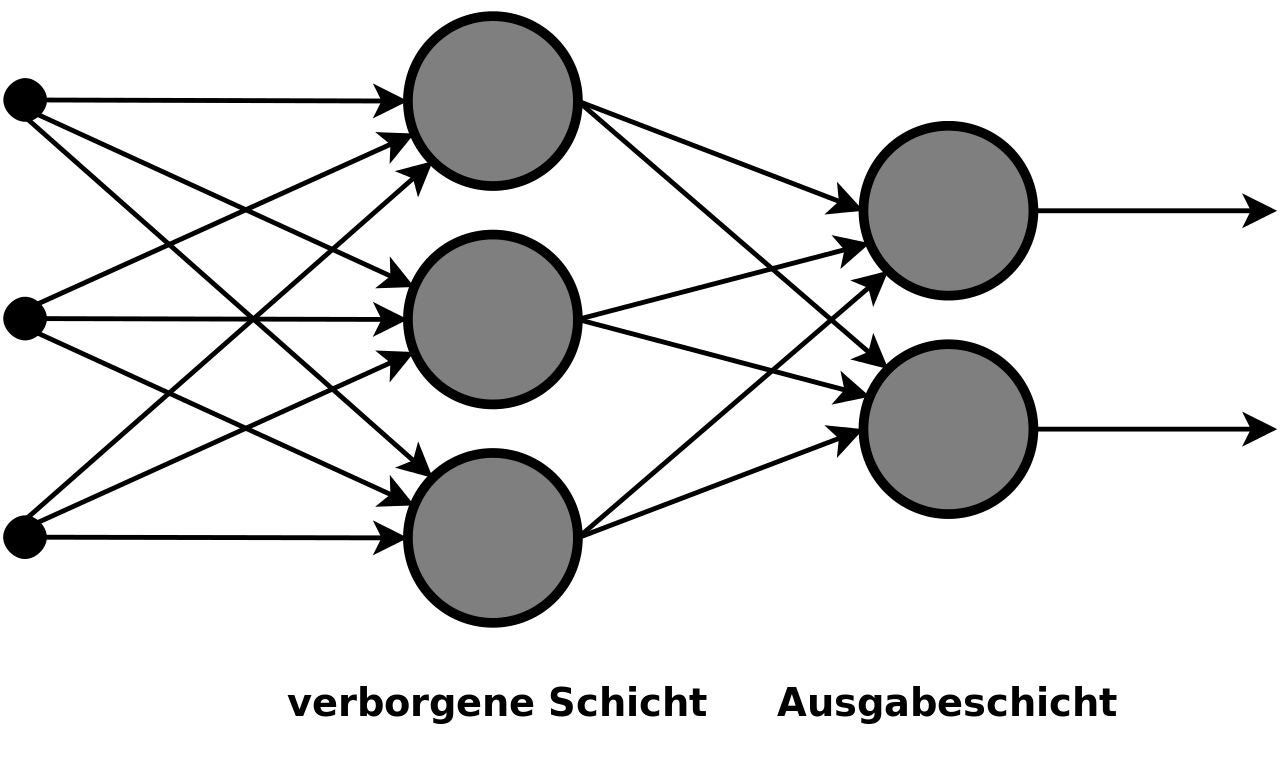
\includegraphics[width=0.5\textwidth]{Bilder/AufbauNN.png}
	\caption{Schematische Darstellung eines neuronalen Netzes \cite{noauthor_kunstliche_nodate}}
    \label{fig:neuronalesNetz}
\end{figure}



\clearpage
\section{Reinforcement Learning}
Reinforcement Learning ist ein Bereich des maschinellen Lernens, bei welchem ein Agent durch Interaktion mit seiner Umgebung (Environment) lernt, welche Aktionen in welchen Situationen am besten geeignet sind, um ein bestimmtes Ziel zu erreichen. Da ein Agent keine konkrete Vorgehensweise besitzt, versucht er über Trial-and-Error herrauszufinden welche Aktionen zu Belohnungen führen. \\
Bestandteile des RL sind der Agent und die Umwelt. Der Agent bekommt die Informationen der Umwelt übergeben und entscheidet welche Handlungen daraus folgen sollen. Das Environment setzt die Aktionen des Agenten in Handlungen (Aktionen) um und bewertet diese mit numerischen Belohnungen (Rewards). Anhand der erhaltenen Rewards, versucht der Agent seine Aktionen anzupassen, um die zukünftigen Belohnungen zu maximieren. \\
Ein RL-Agent nimmt seine Umgebung als eine Menge an bestimmten Zuständen wahr.
Jeder Zustand enthält eine Vielzahl von Merkmalen, welche für die Entscheidungsfindung relevant sein können.
Als Zustandsraum wird die Menge aller möglichen Zustände bezeichnet.\\
Auf jedem dieser Zustände ist es möglich eine bestimmte Menge an Aktionen auszuführen, welche das Umfeld in einen anderen Zustand überführen.
Die Menge aller möglichen Aktionen wird als Aktionsraum bezeichnet.\\
Wird eine Aktion auf einem bestimmten Zustand ausgeführt, so bezeichnet man die Zustandsübergänge bei Ausführung der Aktion als Zustandsübergangsfunktion.\\
Die Verhaltensstrategie  eines Agenten liefert zu jedem Zustand eine Aktion. Die Policy wird im Verlauf des Trainings erlernt.\\
Das Erlernen einer Policy erfolgt durch Training des Neuronalen Netzes. Zu Beginn des Trainings werden Kantengewichte des zur trainierenden Neuronalen Netzes zufällig verteilt. Um zu überprüfen ob seine Aktionen gut oder schlecht sind, erhält der Agent einen numerischen Rückgabewert, welcher jene Information beinhaltet. Diese numerischen Rückgabewerte werden als Belohnungen (Rewards) bezeichnet. Belohnungen werden vom Zustandsraum verteilt und können gutes Verhalten des Agenten durch positive Rewards und falsches Verhalten durch negative Rewards bestärken.
Der Agent versucht den Wert der erhaltenen Belohnungen zu maximieren und erlernt auf diese Weise eine optimale Policy. \\
\newpage
Probleme, welche beim RL auftreten können, sind unter anderem:  
\begin{itemize}
    \item Überanpassung 
    \item Belohnungsumgehung, 
    \item Sparse Rewards
    \item große Beobachtungsvektoren
\end{itemize}
Von \textbf{Überanpassung} spricht man, wenn der Agent ein Problem gut in der Lernumgebung, in welcher er trainiert wurde, lösen kann, allerdings nicht auf abweichenden Umgebungen. Es tritt auf, wenn der Agent zu spezialisiert auf seine Trainingsumgebung ist und sich nicht an andere Situationen anpassen kann. Diese Problem lässt sich durch Generalisierung des Trainingsprozesses beheben. Ein Agent, welcher in vielen zufällig generierten Umgebungen trainiert, kann deutlich besser mit neuen Situationen umgehen, benötigt im Gegenzug dazu auch mehr Zeit zum Trainieren. \cite{zhang_study_2018} \\
\textbf{Belohnungsumgehung} tritt auf, wenn der Agent lernt die Belohnungsfunktion zu manipulieren, um erhaltene Belohnungen zu maximieren, ohne das eigentliche Ziel der Aufgabe zu erreichen. Dies führt zu unerwünschtem Verhalten des Agenten. Verhindert werden kann dieses Problem, indem Belohnungen direkt mit dem Ziel verknüpft werden, also nur Belohnugnen ausgelöst werden, wenn tatsächlich positive Aktionen ausgeführt werden. \cite{pan_effects_2022} \\
Von \textbf{Sparse Rewards} spricht man, wenn die Lernumgebung dem Agenten nur selten oder unregelmäßig Belohnungen vergibt. Dies führt dazu, dass der Agent Schwierigkeiten hat, die ihm gegebene Aufgabe richtig zu erlernen. Um dieses Problem zu umgehen, kann man zusätzliche künstliche Belohnungen einführen, welche den Agenten auf den Weg zum richtigen Verhalten führen. Dies kann im Rückschluss jedoch wieder zur Belohnungsumgehung führen, wenn der Agent die Zwischenbelohnungen, nutzt um maximale Belohnungen zu erhalten. \cite{hare_dealing_2019} \\
Auch ein zu \textbf{großer Beobachtungsvektor} kann zu Komplikationen führen. Wird dem Agenten eine Vielzahl an Observationen zugeführt, müssen erheblich mehr Parameter im Modell verarbeitet werden, was zu größerem Berechnungsaufwand führt. Dadurch wird auch die Lerngeschwindigkeit verlangsamt und der Bedarf an Speicherplatz für die Modelle steigt. So ist es möglich, dass einfach erscheinende Aufgaben mehrere Tage an Rechenzeit benötigen, um ein gutes Modell zu generieren.
\cite{zai_einstieg_2020}

\newpage
\subsection{Markov Entscheidungsprozess}
Jedes RL Problem lässt sich durch den Markov Entscheidungsprozess (= MDP) beschreiben.
Der MDP ist ein mathematisches Modell für Entscheidungsprobleme, bei welchem der Agent abhängig von der Umwelt Entscheidungen trifft, um ein bestimmtes Ziel zu erreichen.
MDP setzen die Einhaltung der Markov-Eigenschaft vorraus. Diese ist erfüllt, wenn ein Zustandsübergang nur vom letzten Zustand und der letzten Aktion abhängig ist.
Hauptkomponenten des MDP sind eine endliche Menge valider Zustände, eine endliche Menge valider Aktionen, Belohnungsfunktion und Verhaltensstrategie.
Das Ziel eines MDP ist es eine optimale Policy, durch Maximierung der erhaltenen Belohnungen, zu ermitteln. \\
\ref{fig:markov} stellt den Ablauf eines MDP dar. Zu Beginn einer Episode befindet sich die Lernumgebung in einem gewissen Zustand. Dieser Zustand wird dem Agenten übergeben. Anhand der Beobachtungen führt der Agent eine Aktion aus, welche die Umgebung verändert. Die Veränderung der Umgebung erzeugt einen neuen Zustand, welcher im nächsten Schritt wiederum dem Agenten übergeben wird. Durch Auslösen von Aktionen in der Lernumgebung werden Belohnungen erzeugt, welche dem Agenten einen numerischen Wert liefern, ob die Aktion gut oder schlecht war. Der Agent versucht die erhaltenen Belohnungen zu maximieren.
Eine hohe Belohnung impliziert das richtige Verhalten zum Lösen des Problems, welches der Agent bewältigen muss.
Dieser Prozess wiederholt sich, bis das Problem gelöst wurde. \cite{zai_einstieg_2020}

\begin{figure}[!h]
	\centering
	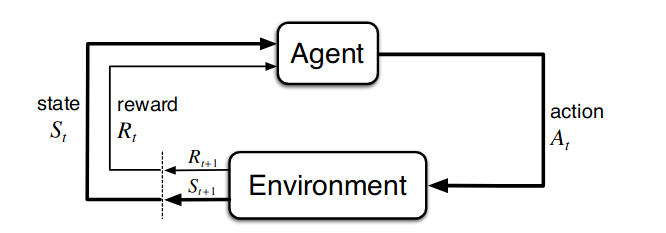
\includegraphics[width=0.7\textwidth]{Bilder/Markov.png}
	\caption{Ablauf eines MDP \cite{sutton_reinforcement_2014}}
	\label{fig:markov}
\end{figure}

\newpage
\section{Das Würfelspiel: Noch Mal}
Im modellierten Spiel 'Noch Mal!' geht es darum so viele Kästchen wie möglich anzukreuzen und damit viele Spalten und gleichfarbige Kästchen auszufüllen. Jeweils ein Farb- und ein Zahlenwürfel müssen kombiniert werden, um entsprechend verfügbare und zusammenhängende Felder der gewählten Farbe abzukreuzen. Dabei kann der Zahlenwürfel die Werte von eins bis fünf oder einen Zahlenjoker ergeben. Der Farbwürfel besitzt die fünf Farben des Feldes und einen Farbjoker. Gespielt wird nach folgenden Regeln:
\setlist{noitemsep}
\begin{enumerate}
    \item Felder in der Spalte H sind von Beginn an verfügbar
    \item Alle Kreuze müssen immer zusammenhängend in genau einem Farbblock der gewählten Farbe platziert werden
    \item Kreuze müssen waagerecht oder senkrecht benachbart zu einem bereits abgekreuzten Feld oder Teil der Spalte H sein, um verfügbar zu werden
    \item Es müssen genau so viele Felder angekreuzt werden, wie das Ergebnis des gewählten Zahlenwürfels
    \item Es könnte nicht mehr als 5 Kästchen in einem Zug abgekreuzt werden
    \item Wird ein Zahlenjoker gewählt, darf der Spieler eine Zahl von 1-5 bestimmen
    \item Wird ein Farbjoker gewählt, darf der Spieler eine Farbe bestimmen
\end{enumerate}

\begin{figure}[!h]
	\centering
	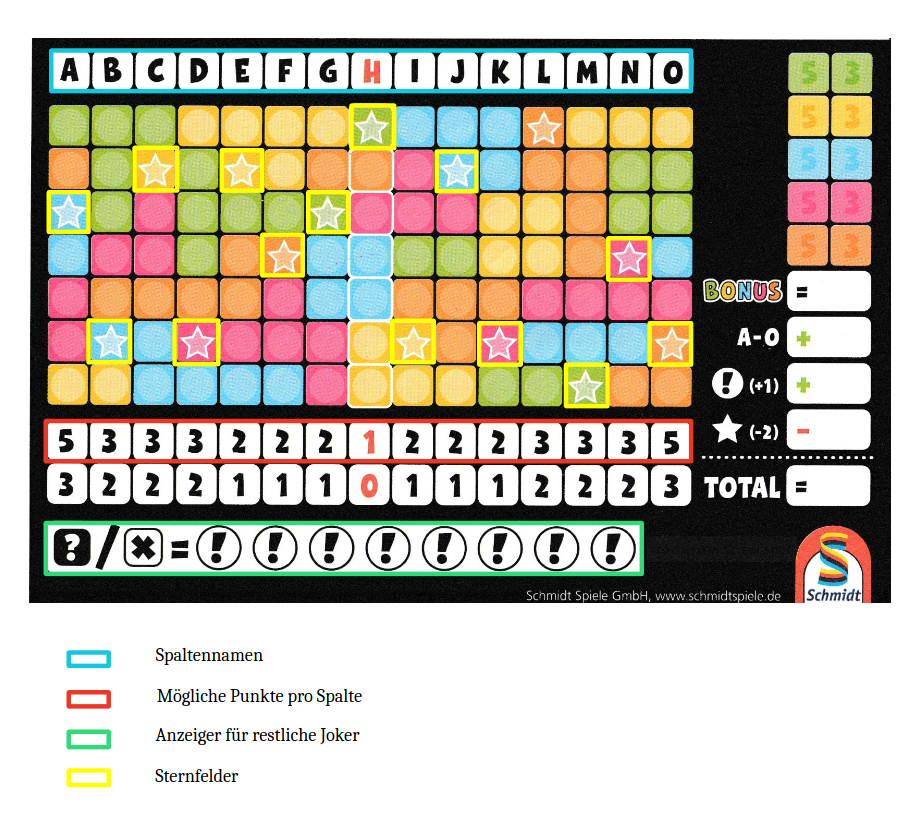
\includegraphics[width=0.7\textwidth]{Bilder/Abbildung2.png}
	\caption{Vorlage des schwarzen Spielfeldes mit Indikation der Punktewertung 
	\cite{schmidt_spiele_gmbh_spielregeln_nodate}}
	\label{fig:Vorlage}
\end{figure}

\begin{figure}[!h]
	\centering
	\includegraphics[width=0.7\textwidth]{Bilder/Beispielzüge.jpg}
	\caption{Beispiele für korrektes und falsches Ankreuzen aus der Spielanleitung 
	\cite{schmidt_spiele_gmbh_spielregeln_nodate}}
	\label{fig:Beispiel}
\end{figure}

Die Grafik \ref{fig:Vorlage} ist ein Spielfeld aus 'Noch mal!'. Nach Vorlage dieses Spielfelds wurde die Lernumgebung für den Agenten modelliert. Die blau markierten Felder geben den Spaltennamen der Spalten an. Die rot markierten Felder zeigen an, wie viele Punkte beim Ausfüllen der jeweiligen Spalte erzielt werden. Das grün markierte Feld zeigt die Anzahl der verbleibenden Joker an, wird ein Joker benutzt, muss eines der Felder abgestrichen werden. Zum Ende des Spiels erhält der Spieler Extrapunkte für die verbleibenden Joker. In jeder Spalte befindet sich ein gelb markiertes Sternfeld. Diese geben zum Ende des Spiels Minuspunkte, weshalb es wichtig ist alle Sternfelder auszufüllen. Abbildung \ref{fig:Beispiel} zeigt Beispiele für korrektes und fehlerhaftes Ankreuzen.


\clearpage


\subsection{Spielablauf Einspielervariante}
Der Spieler hat 30 Züge Zeit maximale Punkte zu erreichen und würfelt jede Spielrunde alle 4 Würfel, bestehend aus 2 Farb- und 2 Zahlenwürfeln. Anschließend wählt er ein Paar aus Farb- und Zahlenwürfel aus und kreuzt entsprechend des gewürfelten Paares verfügbare Felder auf dem Spielfeld ab.
Ein Spieler darf immer entscheiden, ob er Würfelwürfe zum Ankreuzen verwenden möchte oder nicht.
Um Kästchen anzukreuzen, wählt der Spieler eine Kombination aus Zahlen- und Farbwürfel aus. Wählt er beispielsweise 'Grün' und '2' so müssen 2 zusammenhängende grüne Felder angekreuzt werden. \\
Gelingt es dem  Spieler eine Spalte komplett auszufüllen, erhält er je nach Spalte Punkte dafür. Für äußere Spalten werden mehr Punkte vergeben als für die inneren Spalten.
Für das komplette Ausfüllen einer Farbe erhält der Spieler fünf Punkte pro ausgefüllter Farbe. Eine Farbe gilt als komplett ausgefüllt, wenn jedes Feld dieser Farbe abgekreuzt wurde.
Jedes nicht angekreuzte Sternfeld gibt zum Spielende zwei Minuspunkte.
Für jeden übrig gebliebenen Joker erhält der Spieler zum Ende des Spiels einen Punkt.\\
\ref{fig:Punkteübersicht} ist aus der Spielanleitung des Spiels. Sie zeigt an, wie viele Punkte erreichbar sind und bewertet das Ergebnis. Anhand dieser erreichten Punkte wird die Güte des Trainingsfortschritts bewertet.

\begin{figure}[!h]
	\centering
	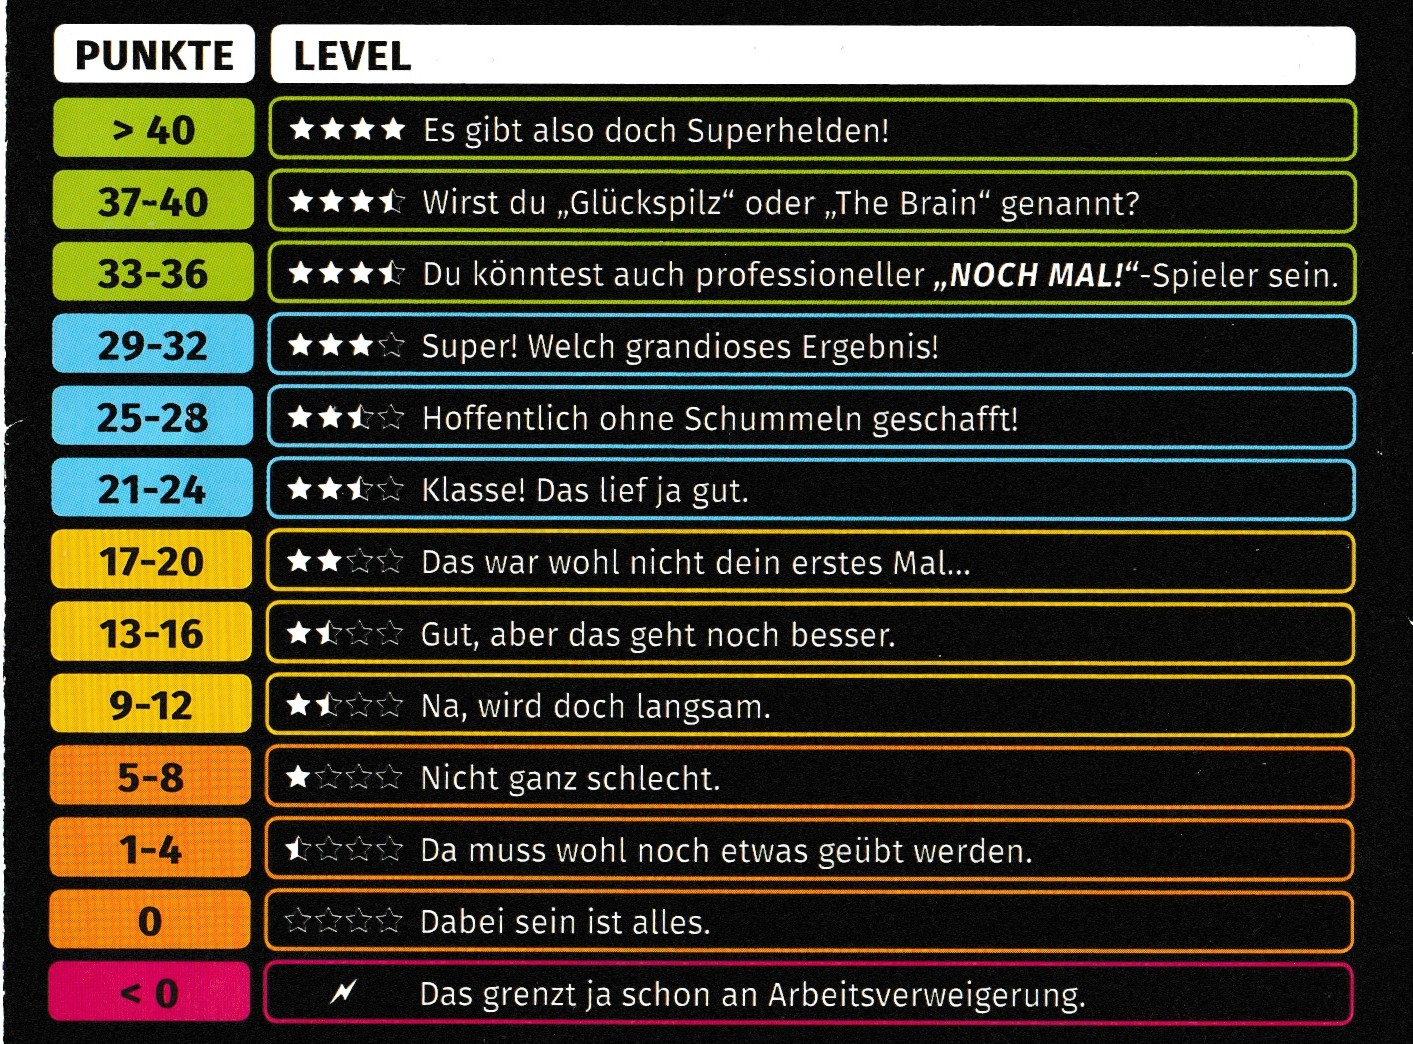
\includegraphics[width=0.5\textwidth]{Bilder/Punkte.jpeg}
	\caption{Grafik zur Bewertung der gesammelten Punkte der Einspieler Variante 
	\cite{schmidt_spiele_gmbh_spielregeln_nodate}}
	\label{fig:Punkteübersicht}
\end{figure}


\newpage 

Um im Spiel 'Noch mal' eine möglichst hohe Anzahl an Punkten zu erhalten, ist es wichtig nach folgenden Strategien zu spielen:\\
\textbf{Priorisierung äußerer Spalten}: Äußere Spalten geben mehr Punkte, weshalb es wichtig ist diese komplett auszufüllen. \\
\textbf{Beenden von Farben}: Vollständig ausgefüllte Farben geben viele Extrapunkte. Eine Farbe gilt als vollständig ausgefüllt, wenn kein Feld dieser Farbe mehr vorhanden ist. Im späten Spielverlauf kann es besser sein Farben komplett zu füllen anstatt Spalten zu werten. \\
 \textbf{Priorisieren von Sternfeldern}: Jedes ausgefüllte Sternfeld gibt 2 Punkte, eine gute Spielweise ist es so viele Sternfelder wie möglich auszufüllen. \\
\textbf{Strategische Nutzung von Jokern}: Ungenutzte Joker geben zum Ende des Spiels Punkte. Es ist gut diese so wenig wie möglich zu nutzen, um Extrapunkte zu bekommen. Jedoch können mit Hilfe von Jokern einfach bestimmte Felder gewählt werden, welche benötigt werden, um eine Wertung zu erzielen. 


%##########################################################
% Drittes Kapitel
%##########################################################
%!TeX root = ./../MusterAbschlussarbeit.tex

%##########################################################
% Inhalt
%##########################################################
\clearpage
\chapter{Konzeption}
\section{Anforderungsanalyse}
In dieser Arbeit soll das Spiel 'Noch mal!' implementiert und von einem RL Agenten gespielt werden. Das Spiel muss nicht vom Nutzer selbst spielbar sein, sondern dem Agenten lediglich eine Lernumgebung bereitstellen, in welcher er trainieren kann. Es müssen alle Funktionalitäten des Spiels abgedeckt werden. Weiterhin muss die Lernumgebung das Durchführen von illegalen Zügen unterbinden. Spielparameter müssen konfigurierbar sein, um die Flexibilität des Trainings zu erhöhen.\\
Die Visualisierung des Spiels steht nicht im Vordergrund. Trotzdessen soll sie vorhanden sein, da sie ermöglicht, Verhaltensweisen des Agenten besser überwachen zu können. Um das Spiel zu programmieren, wird eine leistungsfähige Gameengine vorrausgesetzt, welche die Umsetzung vereinfacht. Da der Lernprozess des Agenten im Vordergrund steht, wird eine benutzerfreundliche Schnittstelle vorrausgesetzt, welche ein RL Framework bereit stellt und die Verwaltung von Modellen vereinfacht. Um das Training zu überwachen und verschiedene Modelle miteinander zu vergleichen, wird ein Framework benötigt, welches den Trainingsprozess grafisch darstellt. Dieses soll ohne großen Mehraufwand nutzbar sein. Das Training von RL Modellen benötigt viel Rechenzeit. Deshalb ist es nötig Traningsprozesse zu parallelisieren, um die Dauer des Trainings zu minimieren. Die Parallelisierung sollte von der Entwicklungsumgebung bereitgestellt werden. Um verschiedene Trainingsszenarien zu erstellen und situativ einsetzen zu können, ist es notwendig mehrere Lernumgebungen konfigurieren und speichern zu können. 
In \ref{tab:requirements} werden die Anforderungen zusammengefasst und in funktionale und nicht funktionale Anforderungen kategorisiert.

    \begin{table}[h]
        \centering

        \label{tab:requirements}
        \begin{tabular}{|l|p{10cm}|}
        \hline
        \textbf{Funktional} & \textbf{Nicht-funktional} \\
        \hline
        Implementierung des Spiels & Überwachen des Trainings \\
        \hline
        Bereitstellen der Lernumgebung & Parallelisierung des Trainingprozesses \\
        \hline
        Abdecken der Spielfunktionalitäten & Konfigurierbare und speicherbare Lernumgebungen \\
        \hline
        Unterbinden von illegalen Spielzügen & Visualisierung des Spiels \\
        \hline
        Schnittstelle für RL-Framework & Verwendung einer leistungsfähigen Gameengine \\
        \hline
        RL-FrameWork& Benutzerfreundliche Entwicklungsumgebung \\
        \hline
        & Konfigurierbare Spielparameter \\
        \hline
        \end{tabular}
        \caption{Anforderungen an die verwendeten Technologien für die Nutzung von RL-Agenten}
    \end{table}

\section{Auswahl der verwendeten Technologien}
Basierend auf der Anforderungsanalyse ergeben sich Anforderungen an die Technologien, welche verwendet werden. 
Um das Spiel 'Noch mal!' zu programmieren, wurde \textbf{Unity} als bevorzugte Gameengine gewählt. Unity stellt eine Vielzahl von Bibliotheken zur Verfügung und ermöglicht die unkomplizierte Umsetzung der Visualisierung des Spiels. C\# ist die gängige Programmiersprache in Unity, deshalb wird das Projekt in C\# umgesetzt. Mit der Auswahl von Unity als Gameengine ist bereits die Mehrheit der funktionalen Anforderungen aus \ref{tab:requirements} teilweise erfüllt, müssen jedoch programmiertechnisch umgesetzt werden. \\
Für die Erstellung des RL-Agenten wurde das \textbf{ML-Agents} Framework verwendet. Es bietet alle Funktionalitäten zum Übergeben von Beobachtungen an den Agenten und Schnittstellen zum Ausführen von Aktionen im Lernumfeld. Weiterhin ist es möglich Aktionen mit Belohnungen zu bewerten. Durch die Integration von ML Agents wird sichergestellt, dass der Agent den aktuellen Zustand des Spiels richtig übergeben bekommt und darauf reagieren kann. Durch die Nutzung des Frameworks, ist die Schnittstelle für die Nutzung von \textbf{Pytorch} geschaffen. Pytorch wird als RL-Framework eingesetzt und passt während des Trainings die Kantengewichte der NN an.\\
Zur grafischen Darstellung des Trainingsprozesses wurde \textbf{Tensorboard} genutzt. Die Integration erfolgt ohne großen Mehraufwand und bietet die automatisierte Erstellung von Grafiken des Trainingsprozesses. Dies erleichtert die Evaluierung von verschiedenen Modellen. \\ 
Zur Visualisierung der erreichten Punkte der Agenten, wurde Python mit \textbf{Matplotlib} verwendet. Mit Matplotlib ist es möglich grafische Darstellungen von Daten zu erstellen. Mithilfe dieser Grafiken ist es möglich Rückschlüsse auf das Verhalten der Agenten zu führen, beziehungsweise deren Trainingsfortschritte zu bewerten. \\
Mit der Verwendung jener genannten Technologien und Frameworks ist es möglich den Rahmen dieser Arbeit zu bearbeiten und zu bewerten.
In \ref{tab:solveRequirements} wird ersichtlich, welche Anforderung über welche Technologie erfüllt wird. \\


\begin{table}[!h]
    \centering
    \label{tab:solveRequirements}
    \begin{tabular}{|c|c|}
    \hline
    \textbf{Anforderung} & \textbf{Technologie} \\
    \hline
    Implementierung des Spiels & Unity \\
    \hline
    Bereitstellen der Lernumgebung & Unity \\
    \hline
    Abdecken der Spielfunktionalitäten & Unity \\
    \hline
    Unterbinden von illegalen Spielzügen & Unity \\
    \hline
    Schnittstelle für RL-Framework & ML-Agents \\
    \hline
    Überwachen des Trainings & TensorBoard, Matplotlib \\
    \hline
    Parallelisierung des Trainingsprozesses & ML-Agents \\
    \hline
    Konfigurierbare Lernumgebungen & ML-Agents \\
    \hline
    Visualisierung des Spiels & Unity, Matplotlib \\
    \hline
    Benutzerfreundliche Entwicklungsumgebung & Unity \\
    \hline
    Konfigurierbare Spielparameter & Unity \\
    \hline
    RL-Framework & Pytorch \\
    \hline
    \end{tabular}
    \caption{Anforderungen an die Implementierung des Spiels 'Noch mal!' für einen RL-Agenten und die entsprechenden Technologien}
\end{table}





%##########################################################
% Viertes Kapitel
%##########################################################
%!TeX root = ./../MusterAbschlussarbeit.tex

%##########################################################
% Inhalt
%##########################################################

\clearpage
\chapter{Implementierung}
\section{Umsetzung in Unity}
Der \textbf{Controller} stellt alle Funktionalitäten bereit, welche gebraucht werden, um die Lernumgebung zu initialisieren.
Er besitzt Prefabs des Agents, des GameFields und der Würfel und initialisiert diese zum Start.
Weiterhin implementiert der Controller die Funktionalität der Punktevergabe, welche für eine Mehrspielervariante genutzt werden kann.
Der Controller ist das Parent aller anderen Elemente und so ist er das zentrale Element der Steuerung. Auch das wiederholte Rollen der Würfel wird im Controller angestoßen.
Der Controller war hilfreich beim Erstellen paralleler Trainings, da dieser mehrfach in die Szene aufgenommen werden musste, um mehrere Spielfelder, welche gleichzeitig bespielt werden, zu initialisieren.

Der \textbf{NumberDice} implementiert die Logik, welche für das Würfeln und Visualisieren der Zahlenwürfel benötigt wird.
Die Visualisierung funktioniert mit selbst angefertigten Sprites, welche in einem sortierten Array liegen und je nach gewürfelter Zahl initialisiert und gerendert werden.
Beim wiederholten Würfeln, wird das aktuelle Sprite zerstört und ein neues initialisiert.
Damit ist gewährleistet, dass immer das aktuelle Würfelergebnis angezeigt wird.
Die Zahl des Würfels wird als Integer gespeichert, wobei er die Zahlen 1-6 annehmen kann.
Die Zahl '6' entspricht dem Zahlenjoker. \ref{fig:NumberSprites} zeigt die verwendeten Sprites für den Zahlenwürfel. 

\newpage
Wie der Zahlenwürfel, implementiert der \textbf{ColorDice} die Funktionalität des Würfelns der Farben.
Diese werden als String dargestellt und können folgende Werte annehmen:\\ \{'blue', 'green','red', 'yellow', 'orange', 'joker'\}.\\
Zur Visualisierung wird ein Sprite erstellt, welches in der gewürfelten Farbe eingefärbt wird. Ein schwarzes Feld entspricht dem gewürfelten Farbjoker.
Das Einfärben der Sprites wird mittels des Switch-Case Statements in \ref{lst:SetColor} ermöglich. 

Das \textbf{GameField} stellt das tatsächliche Spielfeld dar.
Es implementiert die benötigten Methoden, um die SquareFields zu verwalten und rückzusetzen.
Außerdem wird die Anzahl der Joker in ihm gehalten. \ref{fig:Environment} zeigt neun dieser Spielfelder, welche nach Vorlage von \ref{fig:Vorlage} modelliert wurden.

Funktionalitäten:
\setlist{noitemsep}
\begin{itemize}
	\item  Visualisierung des Spielfeldes
    \item  Aktualisieren der Gruppen aller Felder
    \item  Abkreuzen der Felder
    \item  Berechnen der validen Nachbarn der Felder
    \item  Berechnen der verbleibenden Felder einer bestimmten Farbe
    \item  Rückgabe der validen Felder für die aktuell gewählten Würfel
    \item  Reduzieren der verbleibenden Joker
    \item  Rücksetzen der Felder, um ein neues Spiel zu starten
\end{itemize}

Die \textbf{FieldSquares} stellen die einzelnen Teilfelder des Spielfeldes dar. In Tabelle \ref{tab:Informationen in FieldSquares} wird dargestellt, welche Informationen gehalten werden.
\begin{table}[htbp]
    \centering
    \begin{tabular}{|c|c|c|}
    \hline
    \textbf{Beschreibung} & \textbf{Typ} & \textbf{Wertebereich} \\
    \hline
    Feld ist ein Sternfeld & Boolean & True / False \\
    \hline
    Farbe des Feldes & String & - \\
    \hline
    Feld ist ausgefüllt & Boolean & True / False \\
    \hline
    Feld ist verfügbar & Boolean & True / False \\
    \hline
    Clustergröße & Integer & 1-6 \\
    \hline
    X-Koordinate des Feldes & Integer & 0-14 \\
    \hline
    Y-Koordinate des Feldes & Integer & 0-6 \\
    \hline
    \end{tabular}
    \caption{Übersicht Informationen der Fieldsquares}
    \label{tab:Informationen in FieldSquares}
\end{table}

\section{Visualisierung}
Die Visualisierung des Spielfeldes erfolgt über ein angefertigtes Prefab. In diesem wurden die 105 Kästchen in einem Raster von 15x7 instanziiert und manuell mit den Informationen versehen. Dieses manuell angefertigte Spielfeld wurde als Prefab gespeichert und dient als Umgebung für den Agenten.
Zu Beginn des Spiels werden die Felder instanziiert und in die Farben der hinterlegten Information eingefärbt. Ausgefüllte Kästchen werden grau eingefärbt, diese Funktionalität wird im Fieldsquare Prefab ausgeführt. \ref{fig:Environment} zeigt den Aufbau der Trainingsumgebung. Jedes der Spielfelder besitzt einen eigenen Agenten und ist somit die Lernumgebung für genau einen Agenten. Alle Agenten trainieren gemeinsam ein Modell. Es können beliebig viele weitere Lernumgebungen hinzugefügt werden. Mehrere gleichzeitige Traingsvorgänge bedeuten jedoch wiederum einen höheren Rechenaufwand.


\section{Implementierung des Agenten}
Der Agent ist die Schnittstelle zwischen dem Environment und dem RL.
Dem Agent werden alle nötigen Informationen des Spielfeldes übergeben. Diese werden in ein neuronales Netz übertragen, welches wiederum die Ausgabewerte in einem Vektor zurück an den Agenten leitet.
Anschließend wird der Vektor verarbeitet und die gewählten Aktionen werden ausgeführt.
Für gute Aktionen erhält der Agent positive Rewards, bei schlechten Aktionen wird der Zug übersprungen. \\
Zu Beginn jeder Episode, welche einem Spielzug entspricht, muss dem Agenten der aktuelle Zustand des Feldes übermittelt werden, aus welchem er die bestmögliche Option für einen Zug berechnet. In der ML-Agents Bibliothek gibt es hierfür eine vorgefertigte Methode mit dem Namen CollectObservations. Diese erzeugt einen Observationsvektor \ref{tab:Aufbau Beobachtungen}, zu welchem die Informationen der aktuellen Zustands hinzugefügt werden.
Während des Trainings eines neuronalen Netzes, muss die Größe des Vektors und die Art der Werte gleich bleiben. Deswegen ist es nicht möglich ein Modell auf Spielfeldern mit unterschiedlichen Größen zu trainieren, da sich so die Anzahl der Beobachtungen unterscheiden würden.
\ref{lst:CollectObservations} erstellt anhand der Daten den Vektor aus Beobachtungen und übergibt ihn an den Agenten.


Aufbau der Beobachtungen:
\begin{table}[!htbp]
    \centering
    \begin{tabular}{|c|c|c|c|}
    \hline
    \textbf{Index} & \textbf{Beschreibung} & \textbf{Type} & \textbf{Wertebereich} \\
    \hline
    0 & Anzahl der verbleibenden Joker & Float & $[0 - 1]$ \\
    \hline
    1 & Anzahl der gespielten Runden & Float & $[0 - 1]$ \\
    \hline
    2 & Ergebnis des ersten Zahlenwürfels & Float & $[0 - 1]$ \\
    \hline
    3 & Ergebnis des zweiten Zahlenwürfels & Float & $[0 - 1]$ \\
    \hline
    4-9 & Ergebnis des ersten Farbwürfels & Vector6 (Binary) & $(0, 1)^6$ \\
    \hline
    10-15 & Ergebnis des zweiten Farbwürfels & Vector6 (Binary) & $(0, 1)^6$ \\
    \hline
    16-24 & Informationen für Feld 1 & FeldVektor & - \\
    \hline
    25-33 & Informationen für Feld 2 & FeldVektor & - \\
    \hline
    ... & ... & ... & ... \\
    \hline
    953-961 & Informationen für Feld 105 & FeldVektor & - \\
    \hline
    \end{tabular}
    \caption{Zusammenfassung der Observations und Feldinformationen}
    \label{tab:Aufbau Beobachtungen}
\end{table}
    
\begin{table}[!htbp]
    \centering
    \begin{tabular}{|c|c|c|c|}
    \hline
    \textbf{Stelle im Vektor} & \textbf{Beschreibung} & \textbf{Type} & \textbf{Wertebereich} \\
    \hline
    $k*9+16$ - $k+21$ & Farbe des Feldes $k$ & Vector6 (Binary) & $(0, 1)^6$ \\
    \hline
    $k*9+22$ & Ist Feld $k$ verfügbar & Boolean & True / False \\
    \hline
    $k*9+23$ & Ist Feld $k$ abgestrichen & Boolean & True / False \\
    \hline
    $k*9+24$ & Ist Feld $k$ ein Sternfeld & Boolean & True / False \\
    \hline
    \end{tabular}
    \caption{Aufbau FeldVektor}
    \label{tab:Aufbau Feldvektor}
\end{table}

Anhand der Observations berechnet das neuronale Netz einen Ausgabevektor. Tabelle \ref{tab:Aktionbuffer} zeigt den Aufbau der hier verwendeten Beobachtungen. Mit diesem führt der Agent nun bestimmte Aktionen aus und versucht sein Ergebnis (Rewards) zu maximieren.
Anhand der gesammelten Rewards werden die Kantengewichte des Netzes angepasst, um das bestmögliche Ergebnis zu erreichen.

\begin{table}[!h]
    \centering
   
    \begin{tabular}{|c|c|c|c|}
    \hline
    \textbf{Index} & \textbf{Beschreibung} & \textbf{Typ} & \textbf{Wertebereich} \\
    \hline
    \textbf{1} & Index des gewählten ZahlenWürfels & Integer & 0-1 \\
    \hline
    \textbf{2} & Index des gewählten Farbwürfels & Integer & 0-1 \\
    \hline
    \textbf{3} & Jokerzahl & Integer & 0-4 \\
    \hline
    \textbf{4} & X-Koordinate des gewählten Feldes & Integer & 0-14 \\
    \hline
    \textbf{5} & Y-Koordinate des gewählten Feldes & Integer & 0-7 \\
    \hline
    \textbf{6} &  Action 1 für die Auswahl der Nachbarn & Continuous & - \\
    \hline
    \textbf{7} &  Action 2 für die Auswahl der Nachbarn & Continuous & - \\
    \hline
    \textbf{8} &  Action 3 für die Auswahl der Nachbarn & Continuous & - \\
    \hline
    \textbf{9} &  Action 4 für die Auswahl der Nachbarn & Continuous & - \\
    \hline
    \end{tabular}
    \caption{Index und Beschreibung der Variablen}
    \label{tab:Aktionbuffer}
\end{table}

Das Vergeben von Rewards lehnt sich an die Punktevergabe im Spiel, wie nach Vorlage \ref{fig:Vorlage}, an. Der Agent erhält Belohnungen, wenn er auch Punkte im gespielten Spiel erlangen würde. In \ref{tab:rewards} ist eine Übersicht der Belohnungen. Aus dieser lässt sich ablesen, welche Aktion welchen Reward auslöst.

\begin{table}[!h]
    \centering
    \begin{tabular}{|c|c|}
    \hline
    \textbf{Aktion} & \textbf{Erhaltene Belohnung} \\
    \hline
    Abkreuzen eines Sternfeldes & 2 \\
    Ausfüllen einer kompletten Spalte & 1-5 abhängig der Spalte\\
    Ausfüllen einer kompletten Farbe & 5 \\
    Verbleibende Joker zum Ende des Spiels & 1 / verbleibendem Joker \\
    \hline
    \end{tabular}
    \caption{Belohnungen für bestimmte Aktionen}
    \label{tab:rewards}
\end{table}



\clearpage
\section{Spezifikation des Alghorithmus}
Im Folgenden wird der Ablauf zum Wählen der Felder erläutert. Im Beispiel wird der Ausgabevektor \textbf{(1 , 1 , 0 , 3 , 4 , 0.6 , 0.5 , 0.4 , 0.8)} verwendet. \\
Die ersten beiden Stellen des Ausgabevektors entsprechen den gewählten Würfeln.
Im ersten Schritt werden alle Felder des Spielfelds untersucht, ob sie ein valides Ziel für das gewürfelte Ergebnis bilden. Dies ergibt sich aus der Gruppe der Spielfelder, der Farbe und ob das Kästchen verfügbar ist. \ref{lst:GetAvailableFields}
Valide Felder werden in eine Liste (availableFields) aus Verfügbaren Feldern geschrieben. Abb. \ref{fig:alg1} zeigt den beschriebenen Zustand des Feldes.\\

Abb. \ref{fig:alg2} bildet den nächsten Schritt im Algorhitmus ab.
Es wird geprüft, ob verfügbare Felder vorhanden sind.
Wenn kein Feld verfügbar ist, wird die Episode abgebrochen und der Agent überspringt seinen Zug.
Sofern der Agent ein valides Feld gewählt hat, wird dieses in eine weitere Liste (pickedFields) geschrieben und benachbarte Felder der selben Gruppe werden zurückgegeben. \ref{lst:CalculateNeighbors} \\

Im nächsten Schritt wird jedem der verfügbaren Nachbarn, abhängig der Gesamtanzahl, ein Wertebereich zwischen 0 und 1 zugewiesen, dies wird in \ref{fig:alg3} und \ref{tab:field_ranges} verdeutlicht. Anhand des diskreten Wertes des Ausgabevektors, wird das zugehörige Feld in eine Liste aus den gewählten Feldern geschrieben. \ref{lst:PickField}
\begin{table}[!h]
    \centering
    \begin{tabular}{|c|c|c|}
    \hline
    \textbf{FeldKoordinaten} & \textbf{von} & \textbf{bis} \\
    \hline
    (3,5) & 0 & 0.33 \\
    \hline
    (4,4) & 0.33 & 0.66 \\
    \hline
    (3,3) & 0.66 & 0.99 \\
    \hline
    \end{tabular}
    \caption{Bereiche für bestimmte Felder}
    \label{tab:field_ranges}
\end{table}

Für alle gewählten Felder werden die benachbarten Felder zurückgegeben und der vorherige Schritt wiederholt.
Wenn so viele Felder gewählt, wie erwürfelt wurden, werden die Felder anschließend ausgefüllt und auf Rewards überprüft. Dies wird in Abbildung \ref{fig:alg4} dargestellt.

\begin{figure}[!h]
	\centering
	\includegraphics[width=0.45\textwidth]{Bilder/Erklärung_Alghorhitmus_1.png}
	\caption{Valide Felder für das gewählte Würfelergebnis wurden markiert}
    \label{fig:alg1}
\end{figure}

\begin{figure}[!h]
	\centering
	\includegraphics[width=0.45\textwidth]{Bilder/Erklärung_Alghorhitmus_2.png}
	\caption{Feld(3,4) wird in die pickedField Liste aufgenommen und benachbarte Felder werden zurückgegeben.}
    \label{fig:alg2}
\end{figure}


\begin{figure}[!h]
	\centering
	\includegraphics[width=0.45\textwidth]{Bilder/Erklärung_Alghorhitmus_3.png}
	\caption{Feld(4,4) ist das nächste gewählte Feld und wird in pickedFields aufgenommen}
    \label{fig:alg3}
\end{figure}


\begin{figure}[!h]
	\centering
	\includegraphics[width=0.45\textwidth]{Bilder/Erklärung_Alghorhitmus_4.png}
	\caption{Felder wurden gewählt und ausgefüllt}
    \label{fig:alg4}
\end{figure}
\clearpage
\section{Auswertung der erreichten Punkte}
Um die verschiedenen Modelle bewerten zu können, wurden die erreichten Punkte aufgezeichnet und anschließend ausgewertet.
Im Verlauf eines Spiels werden alle erreichten Punkte im Spielfeld gespeichert. 
Nach 30 gespielten Zügen wird die erreichte Punktzahl in eine Logdatei geschrieben.
In \ref{fig:punktWolke} lässt sich ableiten, dass Belohnungen nur dann verteilt werden, wenn es auch zu einer Punktewertung kommt. Die beiden Werte sind lediglich um 30 Punkte verschoben, da der Spieler das Spiel mit -30 Punkten beginnt.

\begin{figure}[!h]
	\centering
	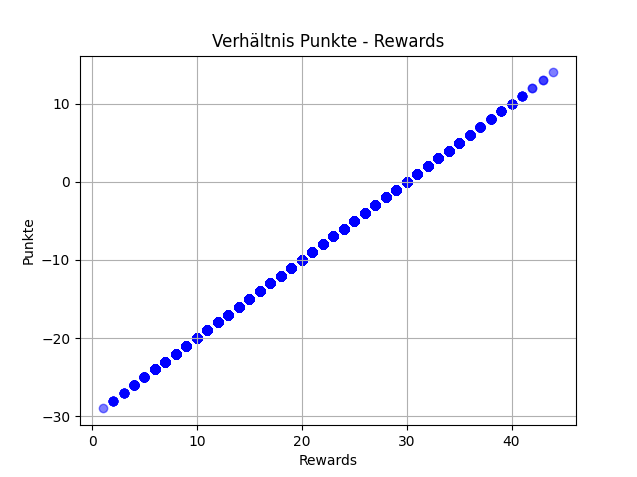
\includegraphics[width=0.45\textwidth]{Bilder/punktWolke.png}
	\caption{Verhältnis Rewards zu Punkten}
    \label{fig:punktWolke}
\end{figure}


Die Logdateien wurden anschließend mit Python ausgewertet. In \ref{lst:ImportLogfiles} werden die angegebenen Punkteaufzeichnugnen importiert und jedem Datensatz ein Titel zur Beschriftung der Graphen hinzugefügt. Im Anschluss wird der gleitende Durchschnitt,abhängig der gewählten Anzahl an Spielen berechnet. 

Dabei werden erst alle Werte addiert und der Mittelwert gebildet. Danach wird der herrausrotierende Wert abgezogen und um den Neuen ergänzt. Auf diese Weise muss jeder Wert lediglich 2 mal gelesen werden. \\ In der Methode \ref{lst:DisplayGraph} können nun variabel Graphen gewählt und anschließend gerendert werden. Vor Methodenaufruf, muss die Liste an anzuzeigenden Graphen bearbeitet werden und in den Methodenaufruf übergeben werden. 





%##########################################################
% Fünftes Kapitel
%##########################################################
%!TeX root = ./../MusterAbschlussarbeit.tex

%##########################################################
% Inhalt
%##########################################################

\clearpage
\chapter{Auswertung und Ausblick}


\section{Bewertung der Ergebnisse}

Probleme 
\section{Schritte zur Verbesserung des Agenten}
More Power und Zeit
Generisches Feld
Babysteps before Supersprints
Besseres Tunen der Hyperparameter
\section{Diskussion}

Dieser Abschnitt stellt den Schlusspunkt der Arbeit dar. In diesem Abschnitt (und im Diskussionteil) erwartet der Leser, 
dass er Antworten auf die in der Einleitung formulierten Fragestellungen findet und sich vergewissert, 
dass diese wirksam verteidigt wurden und mit der von Ihnen formulierten \enquote{These} übereinstimmen.

Die Hauptziele der Diskussion bestehen darin, eine Analyse Ihrer gesammelten Ergebnisse zu präsentieren, 
Ihre Ergebnisse angemessen darzustellen und eine Einschätzung der Bedeutsamkeit Ihrer Arbeit zu geben. Beachten Sie hier,
den Unterschied zur Diskussion im vorherigen Kapitel. Diskutieren Sie hier vor allem den Wert und die Bedeutung Ihrer Ergebnisse, auf Basis der 
Interpretationen aus dem vorherigen Kapitel. Beziehen Sie sich gern auch auf Ihr beschriebenes Problem und Ihr Ziel.

Jede wichtige Schlussfolgerung, die Sie im \enquote{Ergebnisteil} gezogen haben, 
muss hier erneut behandelt werden. Eine gewisse Anzahl von Wiederholungen ist unvermeidlich. Darüberhinaus, 
die Ergebnisse anderer Forschungsarbeiten, müssen mit eindeutigen Verweisen auf auffindbare Literaturquellen versehen sein.

Der Fazit-Teil kann als eine kurze Zusammenfassung Ihrer Diskussion betrachtet werden. 
Der Leser muss sich hier schnell einen Überblick über den Inhalt und die Bedeutung der Arbeit als Ganzes verschaffen.

Dieser Abschnitt soll einen Überblick präsentieren und dient dazu, dem Hauptteil Ihrer Arbeit den letzten Schliff zu geben. 
Die Schlussfolgerung kann auch Hinweise auf ein mögliches zukünftiges Werk enthalten.

\underline{Aber \textbf{mindestens} folgende Punkte}\\
Inhalt des fünften Kapitels (im Allgemeinen):
\begin{itemize}
    \item Reflektieren Sie hier nun die Ergebnisse der Tests aus dem letzten Kapitel
    \item Ordnen Sie diese in den Gesamtkontext ein... gut/schlecht? Was kann man verbessern/anders machen? Schätzen Sie auch ab was Veränderungen bringen könnten.
    \item Was wurde durch die Ergebnisse gezeigt? Geben Sie eine bewertende (selbstkritische) Aussage ab zu Ihrem Schaffen
    \item Geben Sie einen Ausblick was nun folgen sollte/könnte.
\end{itemize}



\lstinputlisting[caption=C-Code Beispiel,label={lst:C-Code-Beispiel},language=C]{Programmcode/test.c}
\lstinputlisting[caption=Python-Code Beispiel,label={lst:Python-Code-Beispiel},language=Python]{Programmcode/test.py}

\textbf{Es ist dabei auch darauf zu achten, dass Quelltexte wenn möglich natürlich nicht über das Seitenende gehen sollten, wie z.B. beim Python-Code Bsp. Setzen Sie daher auch manuell
Seitenumbrüche.} Quelltexte welche eine Seite übersteigen, sind ohnehin eher als Anhang zu betrachten $\rightarrow$ siehe dazu Beschreibung im Anhang.



\lstinputlisting[caption=HTML-Code Beispiel,label={lst:HTML-Code-Beispiel},language=HTML]{Programmcode/test.html}

Nachfolgend noch ein einfaches Beispiel ein Bild einzubinden. Da es sich um Bild\textit{unterschriften} handelt, gehört diese somit \underline{unter} die Abbildung, anders als bei Tabellen\textit{überschriften}.\\
Im \LaTeX-Quelltext sieht man die Optionen für das Einbinden des Bildes. Neben \texttt{scale} wäre auch \texttt{width} möglich mit dem Parameter \texttt{linewidth} oder \texttt{textwidth}.\\
Achten Sie vor allem auf die Lesbarkeit der auf dem Bild befindlichen Informationen, unter der stetigen Annahme, dass es sich um ein ausgedrucktes Dokument handelt. Dort gibt es keinen Zoom.

Empfehlenswert wäre soweit möglich mit skalierbaren Vektorgrafiken zu arbeiten. Allerdings müssten Sie diese vor dem Aufruf von LaTeX in PDFs wandeln (inkscape IM-logo.svg -o IM-logo.pdf) oder Inkscape installieren und LaTeX mit --shell-escape aufrufen.

\begin{figure}[!t]
    \centering
    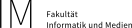
\includegraphics[scale=0.6]{Bilder/logos/IM-logo}
    \caption{Das Logo von Informatik und Medien }
\end{figure}

\begin{figure}[!t]
    \centering
    \includesvg[width=0.6\columnwidth]{Bilder/logos/IM-logo.svg}
    \caption{Das Logo von Informatik und Medien }
\end{figure}

Bedenken Sie bei allen Beschriftungen, egal ob Abbildungen, Tabellen oder Quelltexte, dass Sie, sofern diese nicht Ihrer eigenen Schaffenskraft entsprangen,
diese referenzieren. Im Beispiel der Tabelle \ref{tab:Beispieltabelle} sieht man, dass sich der Beschreibungstext direkt an der Tabelle von dem im Tabellenverzeichnis unterscheidet,
genau um den Punkt der Referenz.


%##########################################################
% Literatur
%##########################################################
%!TeX root = ./../MusterAbschlussarbeit.tex

%##########################################################
% Inhalt
%##########################################################
\printbibliography[title=Literaturverzeichnis,heading=bibintoc]


%##########################################################
% Anhang - nicht verwendete Anhangsseiten bitte kommentieren
%##########################################################
\appendix
\pagenumbering{Roman}
\setcounter{page}{1}

%!TeX root = ./../MusterAbschlussarbeit.tex

%##########################################################
% Inhalt
%##########################################################
\clearpage
\chapter{Anhang - Abbildungen}

Grundsätzlich gehören Tabellen und Abbildungen in den Hauptteil der Arbeit. Hat man aber sehr viele oder auch lange Tabellen, die den Lesefluss im Hauptteil stören würden, dann können diese in einen separaten Anhang aufgenommen werden. Wichtig ist in jedem Fall, dass zwischen Hauptteil und Material im Anhang durch geeignete Verweise eine Beziehung hergestellt wird.

%!TeX root = ./../MusterAbschlussarbeit.tex

%##########################################################
% Inhalt
%##########################################################
\clearpage
\chapter{Anhang - Tabellen}

\relax 
\providecommand{\transparent@use}[1]{}
\providecommand\hyper@newdestlabel[2]{}
\@setckpt{Anhang/AnhangQuelltexte}{
\setcounter{page}{2}
\setcounter{equation}{0}
\setcounter{enumi}{7}
\setcounter{enumii}{0}
\setcounter{enumiii}{0}
\setcounter{enumiv}{0}
\setcounter{footnote}{0}
\setcounter{mpfootnote}{0}
\setcounter{part}{0}
\setcounter{chapter}{0}
\setcounter{section}{0}
\setcounter{subsection}{0}
\setcounter{subsubsection}{0}
\setcounter{paragraph}{0}
\setcounter{subparagraph}{0}
\setcounter{figure}{0}
\setcounter{table}{0}
\setcounter{tabx@nest}{0}
\setcounter{listtotal}{0}
\setcounter{listcount}{0}
\setcounter{liststart}{0}
\setcounter{liststop}{0}
\setcounter{citecount}{0}
\setcounter{citetotal}{0}
\setcounter{multicitecount}{0}
\setcounter{multicitetotal}{0}
\setcounter{instcount}{0}
\setcounter{maxnames}{3}
\setcounter{minnames}{1}
\setcounter{maxitems}{3}
\setcounter{minitems}{1}
\setcounter{citecounter}{0}
\setcounter{maxcitecounter}{0}
\setcounter{savedcitecounter}{0}
\setcounter{uniquelist}{0}
\setcounter{uniquename}{0}
\setcounter{refsection}{0}
\setcounter{refsegment}{0}
\setcounter{maxextratitle}{0}
\setcounter{maxextratitleyear}{0}
\setcounter{maxextraname}{0}
\setcounter{maxextradate}{0}
\setcounter{maxextraalpha}{0}
\setcounter{abbrvpenalty}{50}
\setcounter{highnamepenalty}{50}
\setcounter{lownamepenalty}{25}
\setcounter{maxparens}{3}
\setcounter{parenlevel}{0}
\setcounter{blx@maxsection}{0}
\setcounter{blx@maxsegment@0}{0}
\setcounter{blx@sectionciteorder@0}{8}
\setcounter{mincomprange}{10}
\setcounter{maxcomprange}{100000}
\setcounter{mincompwidth}{1}
\setcounter{afterword}{0}
\setcounter{savedafterword}{0}
\setcounter{annotator}{0}
\setcounter{savedannotator}{0}
\setcounter{author}{0}
\setcounter{savedauthor}{0}
\setcounter{bookauthor}{0}
\setcounter{savedbookauthor}{0}
\setcounter{commentator}{0}
\setcounter{savedcommentator}{0}
\setcounter{editor}{0}
\setcounter{savededitor}{0}
\setcounter{editora}{0}
\setcounter{savededitora}{0}
\setcounter{editorb}{0}
\setcounter{savededitorb}{0}
\setcounter{editorc}{0}
\setcounter{savededitorc}{0}
\setcounter{foreword}{0}
\setcounter{savedforeword}{0}
\setcounter{holder}{0}
\setcounter{savedholder}{0}
\setcounter{introduction}{0}
\setcounter{savedintroduction}{0}
\setcounter{namea}{0}
\setcounter{savednamea}{0}
\setcounter{nameb}{0}
\setcounter{savednameb}{0}
\setcounter{namec}{0}
\setcounter{savednamec}{0}
\setcounter{translator}{0}
\setcounter{savedtranslator}{0}
\setcounter{shortauthor}{0}
\setcounter{savedshortauthor}{0}
\setcounter{shorteditor}{0}
\setcounter{savedshorteditor}{0}
\setcounter{labelname}{0}
\setcounter{savedlabelname}{0}
\setcounter{institution}{0}
\setcounter{savedinstitution}{0}
\setcounter{lista}{0}
\setcounter{savedlista}{0}
\setcounter{listb}{0}
\setcounter{savedlistb}{0}
\setcounter{listc}{0}
\setcounter{savedlistc}{0}
\setcounter{listd}{0}
\setcounter{savedlistd}{0}
\setcounter{liste}{0}
\setcounter{savedliste}{0}
\setcounter{listf}{0}
\setcounter{savedlistf}{0}
\setcounter{location}{0}
\setcounter{savedlocation}{0}
\setcounter{organization}{0}
\setcounter{savedorganization}{0}
\setcounter{origlocation}{0}
\setcounter{savedoriglocation}{0}
\setcounter{origpublisher}{0}
\setcounter{savedorigpublisher}{0}
\setcounter{publisher}{0}
\setcounter{savedpublisher}{0}
\setcounter{language}{0}
\setcounter{savedlanguage}{0}
\setcounter{origlanguage}{0}
\setcounter{savedoriglanguage}{0}
\setcounter{pageref}{0}
\setcounter{savedpageref}{0}
\setcounter{textcitecount}{0}
\setcounter{textcitetotal}{0}
\setcounter{textcitemaxnames}{0}
\setcounter{biburlbigbreakpenalty}{100}
\setcounter{biburlbreakpenalty}{200}
\setcounter{biburlnumpenalty}{0}
\setcounter{biburlucpenalty}{0}
\setcounter{biburllcpenalty}{0}
\setcounter{smartand}{1}
\setcounter{bbx:relatedcount}{0}
\setcounter{bbx:relatedtotal}{0}
\setcounter{svg@param@lastpage}{0}
\setcounter{svg@param@currpage}{-1}
\setcounter{Item}{7}
\setcounter{Hfootnote}{0}
\setcounter{bookmark@seq@number}{0}
\setcounter{lstnumber}{1}
\setcounter{section@level}{1}
\setcounter{lstlisting}{0}
}
Felder wurden gewählt und ausgefüllt

% ***********************************************
\end{document}
% ***********************************************

